\documentclass[utf8, a4paper, 12 pt]{article}
\usepackage{graphicx, float}
\usepackage{fourier}
\usepackage[french]{babel}
\usepackage[T1]{fontenc}
\usepackage[utf8]{inputenc}
\usepackage{enumitem, pifont}
\usepackage{amsmath, amsfonts,amssymb}                                                                                                                                                                                                                                                                                                                                                                                                                                                                                                                                                                                                                                                                                                                                                                                                                                                                                                                                                                                                                                                                                                                                                                                                                                                                                                                                                                                                                                                                                                                                                                                                                                                                                                                                                                                                                                                                                                                                                                                                                                                                                                                                                                                                                                                                                                                                                                                                     

\title{\LARGE \textbf{STATISTIQUES}}
\author{MATH\'EMATHIQUES 4G}
\date{\today}
\setlist[itemize, 1]{label ={\ding{248}}, itemsep = \baselineskip}



\begin{document}

    %\large
    \everymath{\displaystyle}

    \begin{titlepage}
        
        \maketitle
    \end{titlepage}
    
    \setcounter{page}{2}

    \section{Série statistique}
    Une série statistique est une série d'observations, de mesures, de relevés (appelés données ou DATA)%\vspace{1\baselineskip}

    Exemples : \begin{itemize}
        \item les âges des élèves de rhéto de la région bruxelloise (siences sociales)
        \item les noms les plus utilisés par un internaute lors d'une recherche GOOGLE (marketing)
        \item les poids des camemberts PRESIDENT dans un lot (industrie)
        \item les temp\'eratures quotidiennes du mois de mai (m\'et\'eorologie)
        \item les intentions de vote dans une ville aux prochaines \'elections\\ (politique/sondage)
        \item les calories alimentaires d\'epens\'ees au quotidien par les habitants de \\Bruxelles (sant\'e)
    \end{itemize} \vspace{1\baselineskip}

   
    L'objectif est d'analyser ces DATA afin d'en tirer des tendances, des conclusions.
    On note N le nombre total d'observations.
    Ces observations sont, le plus souvent, nombreuses et on range donc d'abord dans des tableaux.

    \section{Les tableaux statistiques}
    %Un tableau de statistique élémentaire s'organise le plus souvent en colonnes.
    Par exemple, on étudie la couleur préférée (=le caractère observé) des élèves de quatrième (=la population).
    Le titre du graphique doit reprendre le caractère observé et la population considérée.\\
    Les intitulés des colonnes sont : \begin{itemize}
        \item les valeurs des caractères observés triés dans l'ordre s'il s'agit de 
        nombres (éventuellement regroupés en intervalles, appelés classes)
        \item les effectifs : le nombre de fois qu'on a obervé chaque valeur du caractère
        \item la fréquence : le pourcentage avec lequel chaque valeur du caractère a été obervée
        \item les fréquences cumulées : voir explication dans l'exercice
        \item des colonnes supplémentaires qui permettent d'effectuer certains calculs 
    \end{itemize} \vspace{1\baselineskip}
    Exercice collectif : créer un tableau de distribution 
    qui correspond à une note d'autoévaluation (sur une échelle de 1 à 10) 
    sur le niveau en mathématiques des élèves de la classe

    \section{Les indicateurs}
    Les indicateurs sont des outils mathématiques qui permettent d'analyser 
    les DATA à partir du tableau de distribution. 
    Dans cette section, nous décrivons quelques-uns d'entre-eux.
    Calculons ensuite ces indicateurs pour notre exemple précédent (exercice).

    \subsection{L'étendue \(E\)}
    L'étendue est la différence entre la plus grande valeur observée et la plus petite.

    \[E = x_{max} - x_{min}\]

    \subsection{Le mode}
    Le mode est la (ou les) valeur(s) du caractère dont l'effectif est le plus grand.

    \subsection{La moyenne \(\overline{x}\)}
    LA moyenne est la somme de toutes les valeurs observées, divisée par le nombre total 
    d'observations.

    \[\overline{x} =\frac{ \sum_{i} {n_i\cdot x_i} }{N}\]

    \subsection{La médiane $M$}
    La médiane est une valeur telle qu'il y ait autant de valeurs inférieures 
    que supérieures à cette valeur.\\
    Pour déterminer la médiane :\begin{itemize}
        \item on range les valeurs par ordre croissant
        \item si N est impair : la médiane est la valeur se situant à la position \(\frac{N+1}{2}\)
        %\item si N est pair, la médiane est la moyenne entre les valeurs se situant à la position \(\frac{N}{2}\) et \(\frac{N+1}{2}\)
    \end{itemize} \vspace{1\baselineskip}
    \subsection{Le premier quartile $Q_1$}
    Le premier quartile est la valeur qui est telle qu'il y ait au moins 25 \% de valeurs inférieures ou égales.\\
    Pour la déterminer le premier quartile :\begin{itemize}
        \item on range les valeurs par ordre croissant
        \item nous calculons  $\frac{N}{4}$\
        \item le premier quartile est l'arrondi par excès de  $\frac{N}{4}$\     
    \end{itemize} \vspace{1\baselineskip}

    \subsection{Le troisième quartile $Q_3$}
    Le troisième quartile est la valeur qui est telle qu'il y ait au moins 75 \% de valeurs inférieures ou égales.\\
    Pour déterminer le troisième quartile :\begin{itemize}
        \item on range les valeurs par ordre croissant
        \item nous calculons  $\frac{3N}{4}$\
        \item le troisième quartile est l'arrondi par excès de  $\frac{3N}{4}$\     
    \end{itemize} \vspace{1\baselineskip}

    \subsection{L'écart-type \(\sigma\)}
    L'écart-type est un nombre qui exprime la dispersion des valeurs observées autour de la moyenne. 
    Pour faciliter ce calcul, on ajoute une colonne à notre tableau.

    \[\sigma = \sqrt{\frac{1}{N} \sum_{i} {n_i ( x_i - \overline{x})^2} }\]


    % \begin{figure}[H]
    %     \centering
    %     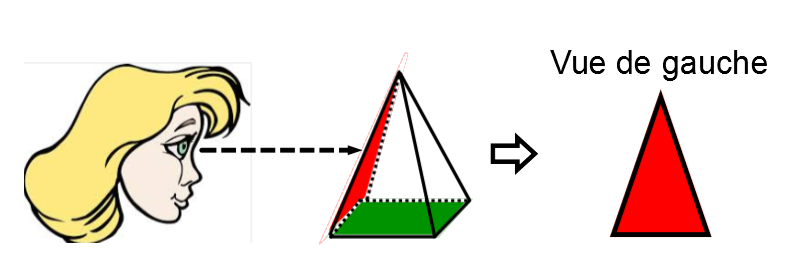
\includegraphics[width = 1\linewidth]{vueGauche.PNG}
    %     \caption[]{Visualiser le solide depuis la gauche}
    % \end{figure}
\end{document}
